% Source printed pp. 225-235 / PDF pp. 233-243.
\section{稳定曲线}\label{src:6.3}
\begin{epigraph}
唯一的问题是巧妙地选择``边界''分支, 即决定允许哪些非一般的簇.
\epigraphauthor{Alan Mayer 和 David Mumford~\cite[3 页]{MM64a}}
\end{epigraph}
Mayer 和 Mumford 在~\cite{MM64a,MM64b} 中引入稳定曲线, 为 $M_g$ 给出具有模意义的紧化, 其中边界 $\overline M_g\setminus M_g$ 上的点对应于奇异稳定曲线.
\subsection{定义与等价条件}\label{src:6.3.1-subsection}
\newterm{$n$-点曲线}{n-pointed curve} 是代数闭域 $k$ 上的曲线 $C$, 配备有序的 $k$-点集 $p_1,\allowbreak \ldots,\allowbreak p_n\in C$; 称 $p_i\in C$ 为\newterm{标记点}{marked point}. 若 $n$-点曲线的点 $q\in C$ 是结点或标记点, 则称其为\textit{特殊点}.
\begin{center}\begin{tikzpicture}
\node[inner sep=0,anchor=south west] (im) at (0,0) {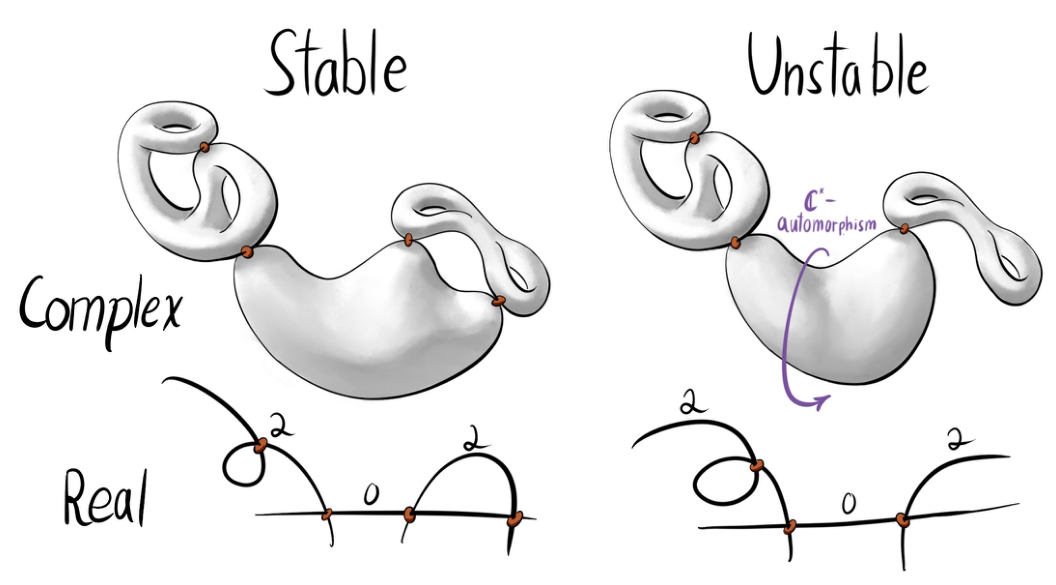
\includegraphics[width=.52\textwidth]{figures/stable-opening.png}};
\begin{scope}[x={(im.south east)},y={(im.north west)}]
\node[fill=white,inner sep=2pt] at (.32,.93) {稳定};
\node[fill=white,inner sep=2pt] at (.76,.93) {不稳定};
\node[fill=white,inner sep=2pt] at (.04,.53) {复};
\node[fill=white,inner sep=2pt] at (.06,.18) {实};
\node[fill=white,inner sep=1pt,font=\tiny,text=violet] at (.77,.69) {$\mathbb C^*$-自同构};
\end{scope}\end{tikzpicture}
\end{center}
% The source omits a caption but begins its numbered statements at 6.3.2.
\setcounter{theorem}{1}
\begin{definition}[稳定, 半稳定与预稳定曲线]\label{src:6.3.2}
代数闭域 $k$ 上亏格为 $g$ 的 $n$-点连通结点射影曲线 $(C,\allowbreak p_1,\allowbreak \ldots,\allowbreak p_n)$ 称为\textit{稳定}的, 若
\begin{enumerate}[(1)]
\item $p_1,\allowbreak \ldots,\allowbreak p_n\in C(k)$ 是互异光滑点,
\item $C$ 不是没有标记点的亏格 $1$ 曲线, 即 $(g,\allowbreak n)\neq(1,\allowbreak 0)$, 且
\item 每条光滑不可约有理子曲线 $\mathbb P^1\subseteq C$ 含有至少 $3$ 个特殊点.
\end{enumerate}
若 (1)--(2) 成立, 且将 (3) 换为每条光滑有理子曲线含有至少 $2$ 个 (而非 $3$ 个) 特殊点, 则称 $(C,\allowbreak p_i)$ 为\textit{半稳定}的. 若仅 (1)--(2) 成立, 则称 $(C,\allowbreak p_i)$ 为\newterm{预稳定}{prestable}的.
\end{definition}
有如下蕴含:
\[
\boxed{\text{稳定}\Rightarrow\text{半稳定}\Rightarrow\text{预稳定}\Rightarrow n\text{-点结点曲线}.}
\]
在无标记点的情形, 曲线是预稳定曲线当且仅当它是结点曲线. 当 $k$ 非代数闭时, 稳定性定义中的条件 (3) 需要调整; 见命题~\bookref{6.3.15}.
\begin{remark}\label{src:6.3.3}
注意若 $(g,\allowbreak n)\in\{(0,\allowbreak 0),\allowbreak (0,\allowbreak 1),\allowbreak (0,\allowbreak 2),\allowbreak (1,\allowbreak 0)\}$, 或等价地 $2g-2+n\leq0$, 则不存在亏格为 $g$ 的 $n$-点稳定曲线. 我们常加上 $2g-2+n>0$ 的条件以排除这些特殊情形.
\end{remark}
\begin{figure}[H]\centering\begin{minipage}[t]{.23\textwidth}\centering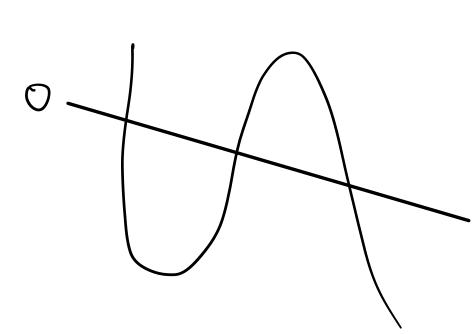
\includegraphics[width=.95\linewidth,height=1.7cm,keepaspectratio]{figures/stable-example-1.png}\\{\small\color{red} 稳定}\end{minipage}
\begin{minipage}[t]{.23\textwidth}\centering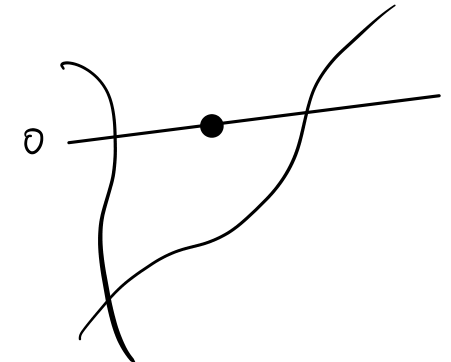
\includegraphics[width=.95\linewidth,height=1.7cm,keepaspectratio]{figures/stable-example-2.png}\\{\small\color{red} 稳定}\end{minipage}
\begin{minipage}[t]{.23\textwidth}\centering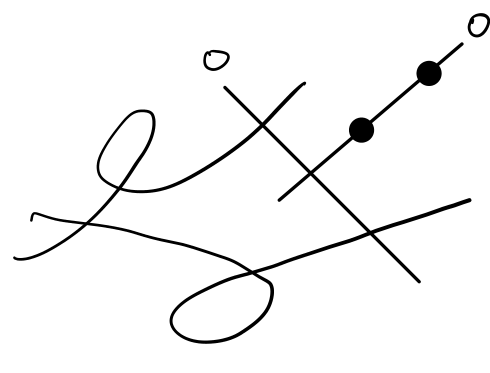
\includegraphics[width=.95\linewidth,height=1.7cm,keepaspectratio]{figures/stable-example-3.png}\\{\small\color{red} 稳定}\end{minipage}
\begin{minipage}[t]{.23\textwidth}\centering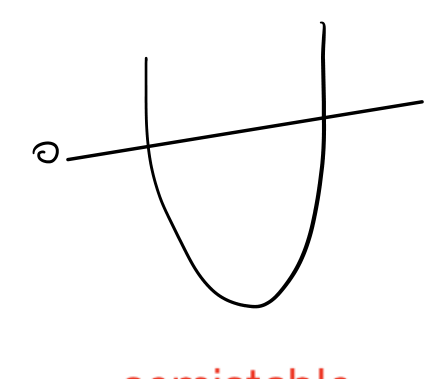
\includegraphics[width=.95\linewidth,height=1.7cm,keepaspectratio]{figures/stable-example-4.png}\\{\small\color{red} 半稳定\\不稳定}\end{minipage}
\medskip\par
\begin{minipage}[t]{.23\textwidth}\centering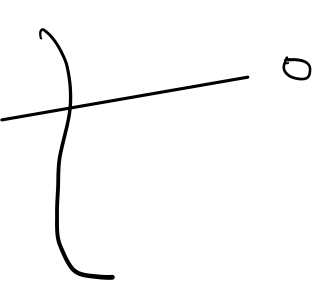
\includegraphics[width=.95\linewidth,height=1.7cm,keepaspectratio]{figures/stable-example-5.png}\\{\small\color{red} 预稳定\\不半稳定}\end{minipage}
\begin{minipage}[t]{.23\textwidth}\centering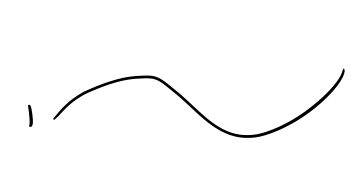
\includegraphics[width=.95\linewidth,height=1.7cm,keepaspectratio]{figures/stable-example-6.png}\\{\small\color{red} 非预稳定}\end{minipage}
\begin{minipage}[t]{.23\textwidth}\centering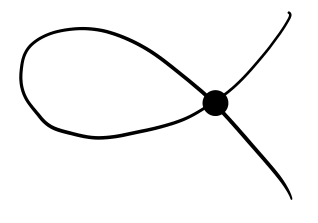
\includegraphics[width=.95\linewidth,height=1.7cm,keepaspectratio]{figures/stable-example-7.png}\\{\small\color{red} 非预稳定}\end{minipage}
\begin{minipage}[t]{.23\textwidth}\centering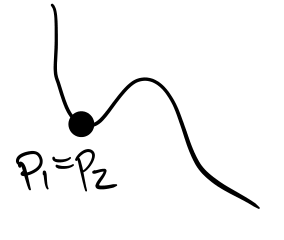
\includegraphics[width=.95\linewidth,height=1.7cm,keepaspectratio]{figures/stable-example-8.png}\\{\small\color{red} 非预稳定}\end{minipage}

\caption{稳定, 半稳定和预稳定曲线的例子.}\label{src:6.3.4}
\end{figure}
稳定曲线 $(C,\allowbreak p_1,\allowbreak \ldots,\allowbreak p_n)$ 的自同构是满足 $\alpha(p_i)=p_i$ 的自同构 $\alpha:C\xrightarrow{\sim}C$. 用 $\operatorname{Aut}(C,\allowbreak p_1,\allowbreak \ldots,\allowbreak p_n)$ 表示自同构的抽象群. 也回顾: 若 $C$ 是亏格 $g\geq2$ 的几何光滑, 连通射影曲线, 则 $\operatorname{Aut}(C)$ 有限 (命题~\bookref{6.1.8}).
\begin{proposition}\label{src:6.3.5}
设 $(C,\allowbreak p_1,\allowbreak \ldots,\allowbreak p_n)$ 是代数闭域 $k$ 上的 $n$-点预稳定曲线. 以下条件等价:
\begin{enumerate}[(1)]
\item $(C,\allowbreak p_1,\allowbreak \ldots,\allowbreak p_n)$ 稳定,
\item $\operatorname{Aut}(C,\allowbreak p_1,\allowbreak \ldots,\allowbreak p_n)$ 有限, 且
\item $\omega_C(p_1+\cdots+p_n)$ 丰沛.
\end{enumerate}
\end{proposition}
\begin{proof}
(1) $\Leftrightarrow$ (2) 由习题~\bookref{6.3.7} 及以下事实得到: 光滑预稳定 $n$-点曲线 $(C,\allowbreak p_i)$ 的自同构群具有正维数, 仅当 $C=\mathbb P^1$ 且 $n\leq2$, 或 $C$ 是亏格 $1$ 曲线且 $n=0$ (见命题~\bookref{6.1.8}). 为证明与 (3) 等价, 使用以下事实: 对子曲线 $T\subseteq C$, 有 $\omega_C|_T=\omega_T(T\cap T^c)$ (习题~\bookref{6.2.21}). 线丛 $\omega_C(p_1+\cdots+p_n)$ 丰沛当且仅当它在每个不可约分支 $T\subseteq C$ 上的限制
\begin{equation}\label{src:6.3.6}
\omega_C(p_1+\cdots+p_n)|_T=\omega_T\left(\sum_{p_i\in T}p_i+(T\cap T^c)\right)
\end{equation}
丰沛. 若 $T$ 的亏格 $g(T)$ 至少为 $2$, 则 $\omega_T$ 丰沛, 因而~\bookeqref{6.3.6} 也丰沛. 若 $g(T)=1$, 则~\bookeqref{6.3.6} 丰沛当且仅当 $n\geq1$ 或 $T$ 与补曲线 $T^c$ 相交. 若 $g(T)=0$, 则~\bookeqref{6.3.6} 丰沛当且仅当 $T$ 含有至少 $3$ 个特殊点.
\end{proof}
\begin{exercise}[带标记的正规化]\label{src:6.3.7}
设 $(C,\allowbreak p_1,\allowbreak \ldots,\allowbreak p_n)$ 是 $n$-点预稳定曲线. 设 $\pi:\widetilde C\to\allowbreak C$ 是正规化, $\widetilde p_i\in\widetilde C$ 是 $p_i$ 的唯一原像, $\widetilde q_1,\allowbreak \ldots,\allowbreak \widetilde q_m\in\widetilde C$ 是结点原像的一个排序. 称 $(\widetilde C,\allowbreak \widetilde p_i,\allowbreak \widetilde q_j)$ 为 $(C,\allowbreak p_i)$ 的\newterm{带标记的正规化}{pointed normalization}. 证明 $(C,\allowbreak p_i)$ 稳定当且仅当 $(\widetilde C,\allowbreak \widetilde p_i,\allowbreak \widetilde q_j)$ 的每个带标记连通分支 (即 $\widetilde C$ 的每个连通分支连同落在其上的 $\widetilde p_i,\allowbreak \widetilde q_j$) 稳定.
\end{exercise}
\begin{exercise}\label{src:6.3.8}
设 $(C,\allowbreak p_1,\allowbreak \ldots,\allowbreak p_n)$ 是 $n$-点预稳定曲线.
\begin{enumerate}[(a)]
\item 证明自同构群概形 $\underline{\operatorname{Aut}}(C,\allowbreak p_i)$ 是代数群.
\item 证明 $\underline{\operatorname{Aut}}(C,\allowbreak p_i)$ 自然是带标记正规化 $(\widetilde C,\allowbreak \widetilde p_i,\allowbreak \widetilde q_j)$ 的自同构群 $\underline{\operatorname{Aut}}(\widetilde C,\allowbreak \widetilde p_i,\allowbreak \widetilde q_j)$ 的闭子群.
\item 证明 $\underline{\operatorname{Aut}}(C,\allowbreak p_i)^0=\underline{\operatorname{Aut}}(\widetilde C,\allowbreak \widetilde p_i,\allowbreak \widetilde q_j)^0$, 但一般有 $\underline{\operatorname{Aut}}(C,\allowbreak p_i)\neq\underline{\operatorname{Aut}}(\widetilde C,\allowbreak \widetilde p_i,\allowbreak \widetilde q_j)$.
\end{enumerate}
\end{exercise}
\paragraph{对偶图.}
\textit{顶点带权的 $n$-标记图} $\Gamma=(G,\allowbreak w,\allowbreak m)$ 是以下数据: 具有顶点集 $V(G)$ 和边集 $E(G)$ 的有限, 连通无向图 $G$ (允许环和重边), 权函数 $w:V(G)\to\mathbb Z_{\geq0}$, 以及 $n$-标记 $m:\{1,\allowbreak \ldots,\allowbreak n\}\to\allowbreak V(G)$. 每个顶点 $m(i)\in V(G)$ 视为一条半边. $\Gamma$ 的亏格是
\[
g(\Gamma)=g(G)+\sum_{v\in V(G)}w(v),
\]
其中 $g(G)=|E(G)|-|V(G)|+1$ 表示 $G$ 的亏格, 即将 $G$ 视为一维 CW 复形时的第一 Betti 数. 若对每个顶点 $v\in V(G)$,
\[
2w(v)-2+\operatorname{val}(v)+|m^{-1}(v)|>0,
\]
则称顶点带权的 $n$-标记图 $\Gamma$ \textit{稳定}. 这里 $\operatorname{val}(v)$ 是 $v$ 的度, 定义为包含 $v$ 的边数, 环计两次. 换言之, 稳定性指对每个顶点 $v$, 以下之一成立: (a) $w(v)\geq2$, (b) $w(v)=1$ 且 $v$ 属于一条边或半边, 或 (c) $w(v)=0$ 且 $\operatorname{val}(v)+|m^{-1}(v)|\geq3$.
\begin{figure}[H]\centering\begin{tikzcd}[column sep=large]
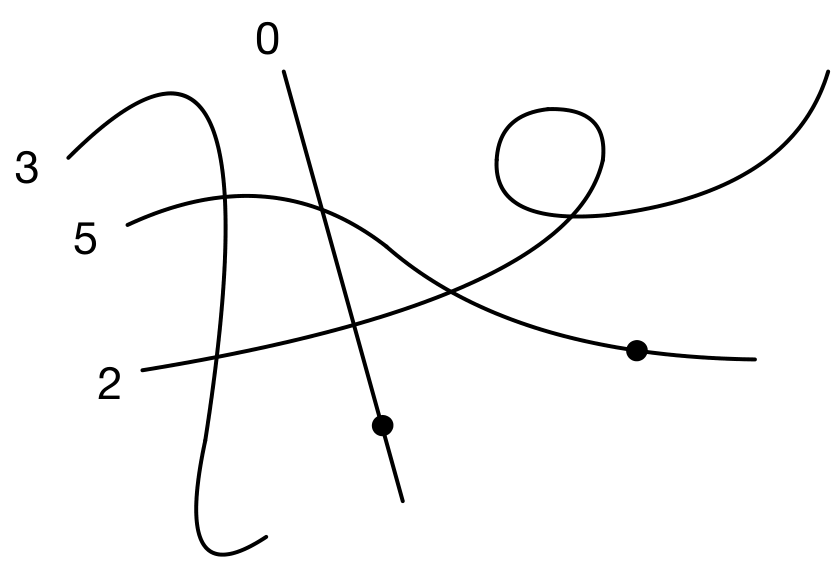
\includegraphics[width=.34\textwidth]{figures/stable-dual-curve.png}\arrow[r,"\text{对偶图}",rightsquigarrow]&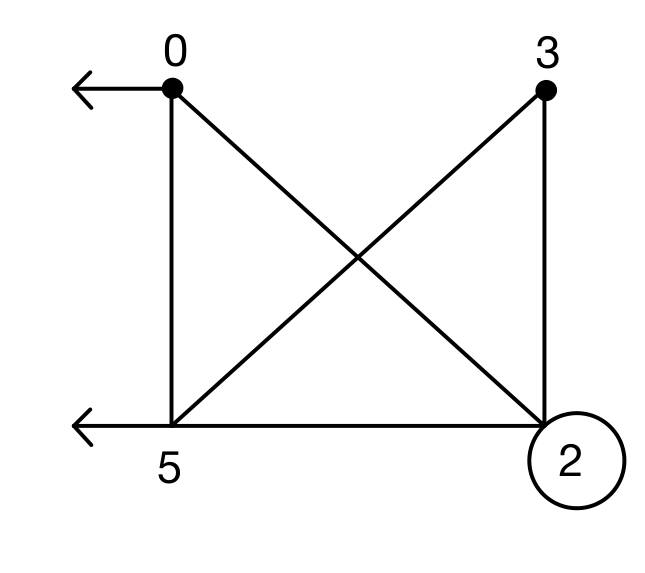
\includegraphics[width=.28\textwidth]{figures/stable-dual-graph.png}
\end{tikzcd}

\begingroup\renewcommand{\thefigure}{6.3.8}\renewcommand{\theHfigure}{6.3.8-figure}\caption{亏格为 $13$ 的曲线及其对偶图.}\label{src:6.3.8-figure}\endgroup
\addtocounter{theorem}{-1}
\end{figure}
\begin{definition}[对偶图]\label{src:6.3.9}
$n$-点预稳定曲线 $(C,\allowbreak p_1,\allowbreak \ldots,\allowbreak p_n)$ 的\newterm{对偶图}{dual graph} 定义为 $\Gamma=(G,\allowbreak w,\allowbreak m)$, 其中 $G$ 的顶点 $v_i$ 对应于 $C$ 的不可约分支 $C_i$, 权 $w(v_i)$ 是 $C_i$ 的几何亏格. 对落在分支 $C_i,\allowbreak C_j$ 上的每个结点 $q$, 有连接 $v_i,\allowbreak v_j$ 的边 $e_q$, 标记 $m(i)$ 是满足 $p_i\in C_j$ 的顶点 $v_j$.
\end{definition}
\begin{exercise}[容易]\label{src:6.3.10}
证明 $n$-点预稳定曲线 $(C,\allowbreak p_i)$ 稳定当且仅当其对偶图 $\Gamma$ 稳定, 且 $C$ 的亏格等于 $\Gamma$ 的亏格.
\end{exercise}
稳定曲线的叠 $\overline{\mathcal M}_{g,\allowbreak n}$ 按对偶图具有一个分层 (习题~\bookref{6.6.23}).
\begin{figure}[H]\centering\begin{tikzcd}[column sep=large,row sep=small]
&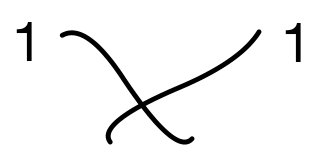
\includegraphics[width=.13\textwidth,height=1cm,keepaspectratio]{figures/stable-g2-curve-2.png}\arrow[r]&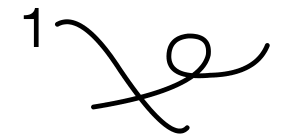
\includegraphics[width=.13\textwidth,height=1cm,keepaspectratio]{figures/stable-g2-curve-3.png}\arrow[r]&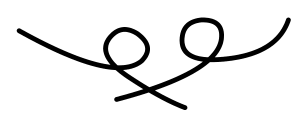
\includegraphics[width=.13\textwidth,height=1cm,keepaspectratio]{figures/stable-g2-curve-4.png}\\
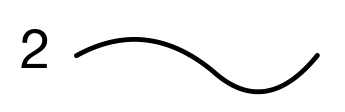
\includegraphics[width=.13\textwidth,height=1cm,keepaspectratio]{figures/stable-g2-curve-1.png}\arrow[ur]\arrow[dr]&&&\\
&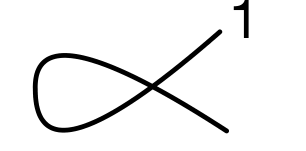
\includegraphics[width=.13\textwidth,height=1cm,keepaspectratio]{figures/stable-g2-curve-5.png}\arrow[r]\arrow[uur]&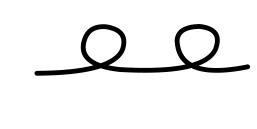
\includegraphics[width=.13\textwidth,height=1cm,keepaspectratio]{figures/stable-g2-curve-6.png}\arrow[r]\arrow[uur]&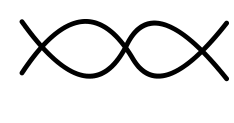
\includegraphics[width=.13\textwidth,height=1cm,keepaspectratio]{figures/stable-g2-curve-7.png}
\end{tikzcd}
\par\smallskip\noindent\rule{.85\textwidth}{.4pt}\par\smallskip
\begin{tikzcd}[column sep=large,row sep=small]
&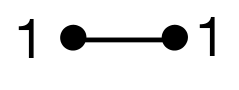
\includegraphics[width=.13\textwidth,height=1cm,keepaspectratio]{figures/stable-g2-graph-2.png}\arrow[r]&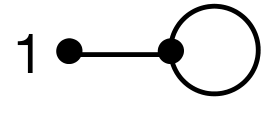
\includegraphics[width=.13\textwidth,height=1cm,keepaspectratio]{figures/stable-g2-graph-3.png}\arrow[r]&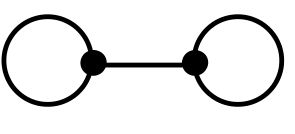
\includegraphics[width=.13\textwidth,height=1cm,keepaspectratio]{figures/stable-g2-graph-4.png}\\
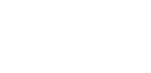
\includegraphics[width=.13\textwidth,height=1cm,keepaspectratio]{figures/stable-g2-graph-1.png}\arrow[ur]\arrow[dr]&&&\\
&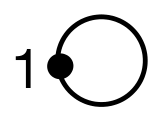
\includegraphics[width=.13\textwidth,height=1cm,keepaspectratio]{figures/stable-g2-graph-5.png}\arrow[r]\arrow[uur]&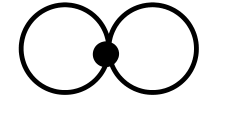
\includegraphics[width=.13\textwidth,height=1cm,keepaspectratio]{figures/stable-g2-graph-6.png}\arrow[r]\arrow[uur]&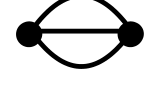
\includegraphics[width=.13\textwidth,height=1cm,keepaspectratio]{figures/stable-g2-graph-7.png}
\end{tikzcd}

\begingroup\renewcommand{\thefigure}{6.3.10}\renewcommand{\theHfigure}{6.3.10-figure}\caption{无标记点的亏格 $2$ 顶点带权图共有七种. 上方显示曲线, 下方显示其对偶图. 箭头表示特殊化. 从左列向右列, $\overline{\mathcal M}_2$ 中参数化具有给定对偶图的曲线的子叠的维数依次为 $3$, $2$, $1$, $0$.}\label{src:6.3.10-figure}\endgroup
\addtocounter{theorem}{-1}
\end{figure}
\begin{exercise}\label{src:6.3.11}
\begin{enumerate}[(a)]
\item 分类亏格为 $1$ 的稳定顶点带权 $2$-标记图.
\item 确定亏格为 $3$ 的稳定顶点带权 $0$-标记图的同构类数.
\end{enumerate}
\end{exercise}
\subsection{有理尾与有理桥}\label{src:6.3.2-subsection}
\begin{definition}[有理尾与有理桥]\label{src:6.3.12}
设 $(C,\allowbreak p_1,\allowbreak \ldots,\allowbreak p_n)$ 是域 $k$ 上的 $n$-点预稳定曲线. 对亏格为 $0$, 且补曲线 $E^c=\overline{C\setminus E}$ 非空的不可约光滑子曲线 $E\subseteq C$, 我们称其为
\begin{itemize}
\item \newterm{有理尾}{rational tail}, 若概形意义的交 $E\cap E^c$ 是单个约化点 $x$, $\mathrm H^0(E,\allowbreak \mathcal O_E)\cong\kappa(x)$, 且 $E$ 不含标记点; 以及
\item \newterm{有理桥}{rational bridge}, 若概形意义的交 $E\cap E^c$ 在 $\mathrm H^0(E,\allowbreak \mathcal O_E)$ 上的次数为 $2$, 且 $E$ 不含标记点; 或者 $E$ 只含一个标记点 $p_j$, 且 $E$ 是 $(C,\allowbreak p_1,\allowbreak \ldots,\allowbreak \widehat p_j,\allowbreak \ldots,\allowbreak p_n)$ 的有理尾.
\end{itemize}
\end{definition}
在代数闭域上, 每条不可约光滑有理子曲线 $E$ 同构于 $\mathbb P^1$. $E$ 是有理尾当且仅当 $E\cdot E^c=1$ 且 $E$ 没有标记点; $E$ 是有理桥当且仅当 $E\cdot E^c=2$ 且 $E$ 没有标记点, 或 $E\cdot E^c=1$ 且 $E$ 恰有一个标记点.
\begin{figure}[H]\centering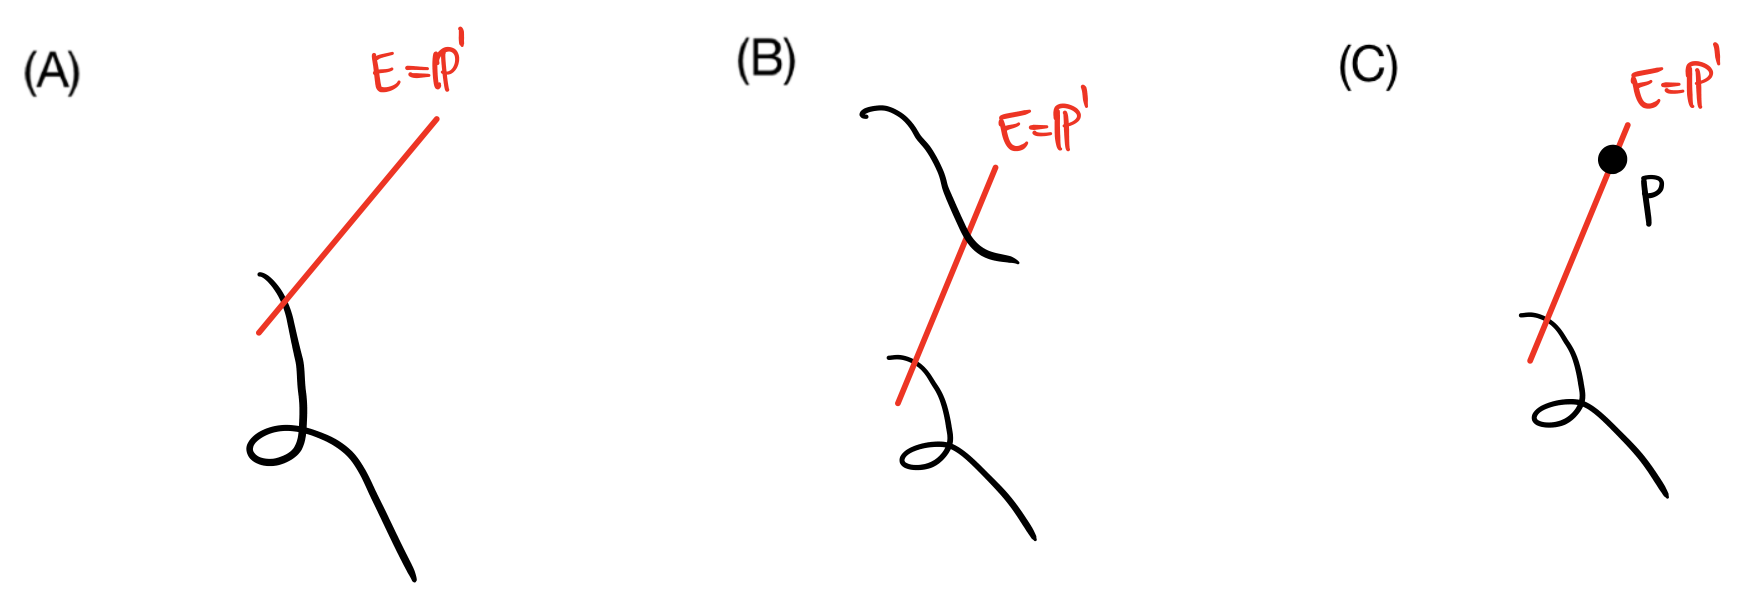
\includegraphics[width=.64\textwidth]{figures/fig-6.3.12.png}
\begingroup\renewcommand{\thefigure}{6.3.12}\renewcommand{\theHfigure}{6.3.12-figure}\caption{(A) 含有一个有理尾, (B) 与 (C) 含有有理桥.}\label{src:6.3.12-figure}\endgroup\addtocounter{theorem}{-1}
\end{figure}
在任意域上, 有理尾和有理桥的分类更为微妙. 考虑到有理曲线的分类也更复杂 (见习题~\bookref{6.1.13} 和~\bookref{6.1.14}), 这并不意外.
\begin{lemma}\label{src:6.3.13}
设 $(C,\allowbreak p_i)$ 是域 $k$ 上的 $n$-点预稳定曲线.
\begin{enumerate}[(1)]
\item 若 $E$ 是有理尾, $k':=\mathrm H^0(E,\allowbreak \mathcal O_E)=\kappa(x)$, 则 $k'$ 是 $k$ 的有限可分域扩张, 且 $E\cong\mathbb P_{k'}^1$.
\item 若 $E$ 是没有标记点的有理桥, 则 $k':=\mathrm H^0(E,\allowbreak \mathcal O_E)$ 是 $k$ 的有限可分域扩张, $k'':=\mathrm H^0(E\cap E^c,\allowbreak \mathcal O_{E\cap E^c})$ 是 $k'$ 的次数为 $2$ 的可分域扩张或 $k''=k'\times k'$.
\end{enumerate}
\end{lemma}
\begin{proof}
两种情形下, 由于 $E$ 约化且连通, $k'=\mathrm H^0(E,\allowbreak \mathcal O_E)$ 是域. 对 (1), 交点 $x=E\cap E^c$ 是结点, 因而 $k'=\kappa(x)$ 是 $k$ 的可分域扩张 (命题~\bookref{6.2.4}). 通过结构映射 $E\to\Spec\Gamma(E,\allowbreak \mathcal O_E)=\Spec k'$ 将 $E$ 视为 $k'$ 上的概形, 由其不可约, 光滑, 亏格为 $0$ 且含有有理点, 得到 $E\cong\mathbb P_{k'}^1$. 对 (2), $E\cap E^c$ 的点是 $C$ 中的结点, 但在 $E,\allowbreak E^c$ 中都是光滑点. 由 $\dim_{k'}k''=2$, 或 $k''$ 是域, 此时由命题~\bookref{6.2.4} 它在 $k$ 上可分; 或 $k''=k'\times k'$.
\end{proof}
\begin{exercise}\label{src:6.3.14}
若 $K/k$ 是域扩张, 则 $(C,\allowbreak p_i)$ 有有理尾 (分别地, 有理桥) 当且仅当 $(C\times_k K,\allowbreak p_i\times_k K)$ 有有理尾 (分别地, 有理桥).
\end{exercise}
稳定性等价于不含有理尾或有理桥.
\begin{proposition}\label{src:6.3.15}
设 $(C,\allowbreak p_i)$ 是域 $k$ 上亏格为 $g$ 的 $n$-点预稳定曲线. 若 $K$ 是包含 $k$ 的代数闭域, 则 $(C\times_k K,\allowbreak p_i\times_k K)$ 稳定 (分别地, 半稳定) 当且仅当 $(C,\allowbreak p_i)$ 不含有理尾或有理桥 (分别地, 不含有理尾).
\end{proposition}
\begin{proof}
在代数闭域上, 稳定 (分别地, 半稳定) 等价于不含有理尾或有理桥 (分别地, 有理尾). 因此结论由有理尾或有理桥的存在性不受域扩张影响这一事实 (习题~\bookref{6.3.14}) 得到.
\end{proof}
\begin{remark}[与 $-1$ 和 $-2$ 曲线的关系]\label{src:6.3.16}
设 $C\to\Delta=\Spec R$ 是 DVR $R$ 上的结点曲线族, 剩余域 $k$ 代数闭, 一般纤维光滑. 若 $E\cong\mathbb P^1\subseteq C_0$ 是中心纤维中的光滑有理子曲线, 则 $E^2=-E\cdot E^c$ (由恒等式 $0=E\cdot C_0=E\cdot E+E\cdot E^c$ 得到). 因而若 $E$ 是有理尾 (分别地, 无标记点的有理桥), 则 $E^2=-1$ (分别地, $E^2=-2$).
\end{remark}
\begin{figure}[H]\centering\begin{tikzcd}[column sep=large,row sep=small]
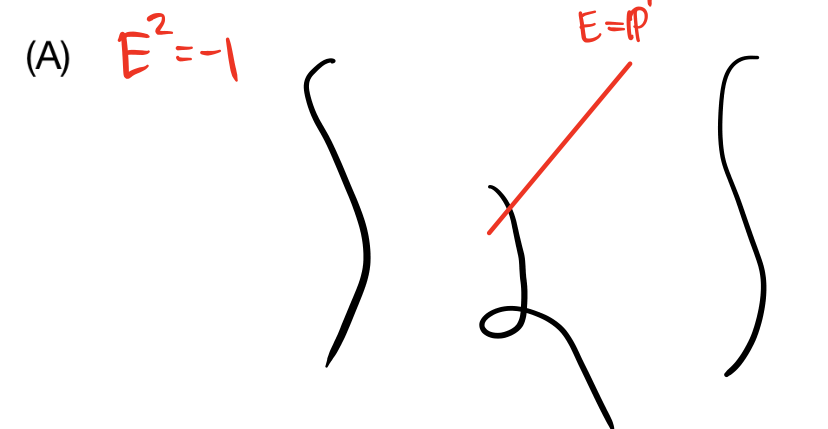
\includegraphics[width=.32\textwidth]{figures/stable-contract-tail-top.png}\arrow[d]&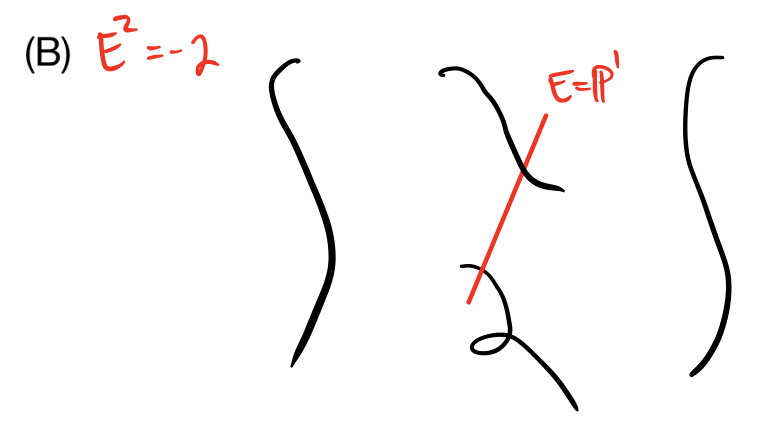
\includegraphics[width=.32\textwidth]{figures/stable-contract-bridge-top.png}\arrow[d]\\
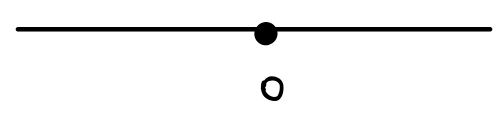
\includegraphics[width=.2\textwidth]{figures/stable-contract-tail-bottom.png}&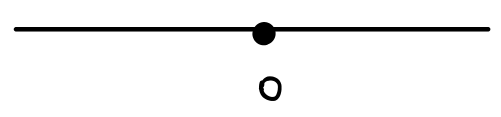
\includegraphics[width=.2\textwidth]{figures/stable-contract-bridge-bottom.png}
\end{tikzcd}

\begingroup\renewcommand{\thefigure}{6.3.16}\renewcommand{\theHfigure}{6.3.16-figure}\caption{在 (A) (分别地, (B)) 中, 例外分支 $E$ 与曲线其余部分在一个点 (分别地, 两个点) 相交, 且 $E^2=-1$ (分别地, $E^2=-2$).}\label{src:6.3.16-figure}\endgroup\addtocounter{theorem}{-1}
\end{figure}
后文预稳定曲线族的稳定收缩 (\bookref{6.6.6}) 将推广以下习题.
\begin{exercise}[困难]\label{src:6.3.17}
设 $C\to\Delta=\Spec R$ 是 DVR $R$ 上的结点曲线族, 一般纤维光滑. 对中心纤维中的任意有理尾或有理桥 $E\subset C_0$, 证明存在 $E$ 的收缩 $C\to\allowbreak C'$, 其中 $C'\to\Delta$ 是结点曲线族.

\textit{提示:} Castelnuovo 收缩定理 (\bookref{B.2.6}) 给出收缩 $C\to\allowbreak C'$ 的存在性. 难点在于说明中心纤维 $C'_0$ 是结点曲线. 可使用极小模型纲领中的事实: $C'_0$ 是结点曲线当且仅当对 $(C',\allowbreak C'_0)$ 是对数典范的~\cite[推论 2.32, 定理 4.9(2)]{Kol13}, 并利用 $(C,\allowbreak C_0)$ (分别地, $(C,\allowbreak C_0-E)$) 是对数典范的, 说明后一性质成立.
\end{exercise}
\subsection{对偶化层的正性}\label{src:6.3.3-subsection}
\begin{exercise}[中等]\label{src:6.3.18}
设 $(C,\allowbreak p_1,\allowbreak \ldots,\allowbreak p_n)$ 是代数闭域 $k$ 上的 $n$-点预稳定曲线, $L:=\omega_C(p_1+\cdots+p_n)$.
\begin{enumerate}[(a)]
\item 若 $(C,\allowbreak p_i)$ 稳定, 证明 $k\geq3$ 时 $L^{\otimes k}$ 甚丰沛, 且 $k\geq2$ 时 $\mathrm H^1(C,\allowbreak (\omega_C(p_1+\cdots+p_n))^{\otimes k})=0$.
\item 对 $k\geq2$, 证明 $(C,\allowbreak p_i)$ 半稳定当且仅当 $L^{\otimes k}$ 无基点.
\end{enumerate}
\textit{提示:} 对 (a), 证明 $L^{\otimes k}$ 的整体截面分离点和切向量, 换言之, 映射
\[
\begin{aligned}
\mathrm H^0(C,L^{\otimes k})&\to(L^{\otimes k}\otimes\kappa(x))\oplus(L^{\otimes k}\otimes\kappa(y)),\\
\mathrm H^0(C,L^{\otimes k})&\to L^{\otimes k}\otimes\mathcal O_{C,x}/\mathfrak m_x^2
\end{aligned}
\]
满射. 利用 Serre 对偶, 并按 $x,\allowbreak y$ 为光滑点或结点分类讨论. 另见~\cite[定理 2]{DM69}, \cite[引理 10.6.1]{ACG11}, \cite[Tag 0E8X]{SP} 和~\cite[命题 13.2.17]{Ols16}.
\end{exercise}
\begin{exercise}[很好的练习]\label{src:6.3.19}
若 $C$ 是亏格分别为 $i$ 和 $g-i$ 的曲线沿单个结点 $p=C_1\cap C_2$ 的结点并 $C_1\cup C_2$, 证明 $\omega_C$ 在 $p$ 处有基点.
\end{exercise}
\subsection{稳定曲线族}\label{src:6.3.4-subsection}
\begin{definition}\label{src:6.3.20}
概形 $S$ 上的\textit{$n$-点曲线族} 是代数空间的固有, 平坦有限表现态射 $C\to\allowbreak S$, 配备 $n$ 个截面 $\sigma_1,\allowbreak \ldots,\allowbreak \sigma_n:S\to\allowbreak C$, 使得每个几何纤维 $C_s$ 都是 $\Spec\kappa(s)$ 上的曲线 (例如一维有限型 $\kappa(s)$-概形).

\textit{$n$-点稳定曲线族} (分别地, \textit{半稳定曲线族}, \textit{预稳定曲线族}, \textit{结点曲线族}) 是每个几何纤维 $(C_s,\allowbreak \sigma_1(s),\allowbreak \ldots,\allowbreak \sigma_n(s))$ 都稳定 (分别地, 半稳定, 预稳定, 结点) 的 $n$-点曲线族.
\end{definition}
\begin{remark}[注意]\label{src:6.3.21}
若 $(C\to\allowbreak S,\allowbreak \sigma_i)$ 是概形 $S$ 上的稳定曲线族, 则 $C\to\allowbreak S$ 必为射影态射 (命题~\bookref{6.3.22}), 因而 $C$ 是概形. 虽然域上每个一维分离有限型代数空间都是概形 (定理~\bookref{5.5.32}), 在相对情形中, 族的总空间 $C$ 却未必是概形. 存在亏格 $0$ 的预稳定曲线族~\cite[例 2.3]{Ful10} 和亏格 $1$ 的光滑曲线族~\cite[XIII.3.2]{Ray70}, 其总空间不是概形; 另见例~\bookref{3.1.16}. 下一节将证明所有曲线 (分别地, 结点曲线, 半稳定曲线, 预稳定曲线) 的叠是代数叠, 特别地满足曲线族的下降条件; 该结果要求允许族的总空间为代数空间.
\end{remark}
对 $n$-点曲线族 (分别地, 结点曲线族), 不要求标记点互异或落在 $C\to\allowbreak S$ 的相对光滑轨迹上. 对稳定, 半稳定和预稳定曲线族, 标记点互异且避开结点. 若 $(C\to\allowbreak S,\allowbreak \sigma_i)$ 是 $n$-点预稳定曲线族, 则 $C\to\allowbreak S$ 是局部完全交态射. 因而有相对对偶化线丛 $\omega_{C/S}$, 与基变换 $T\to\allowbreak S$ 相容, 特别地, 在 $C\to\allowbreak S$ 的每个纤维上限制为对偶化线丛 $\omega_{C_s}$; 见~\cite{Har66c} 或~\cite[\S 6.4]{Liu02}. 每个截面 $\sigma_i$ 的像是包含在光滑轨迹中的除子, 可形成线丛 $\omega_{C/S}(\sigma_1+\cdots+\sigma_n)$.

以下陈述将命题~\bookref{6.3.5} 推广到曲线族. 用 $\underline{\operatorname{Aut}}(C/S,\allowbreak \sigma_1,\allowbreak \ldots,\allowbreak \sigma_n)$ 表示参数化 $n$-点预稳定曲线族的自同构的 $S$ 上局部有限型群概形.
\begin{proposition}\label{src:6.3.22}
设 $(C\to\allowbreak S,\allowbreak \sigma_i)$ 是概形 $S$ 上亏格为 $g$ 的 $n$-点预稳定曲线族. 以下条件等价:
\begin{enumerate}[(1)]
\item $(C\to\allowbreak S,\allowbreak \sigma_i)$ 是稳定曲线族,
\item $\underline{\operatorname{Aut}}(C/S,\allowbreak \sigma_1,\allowbreak \ldots,\allowbreak \sigma_n)\to\allowbreak S$ 拟有限, 且
\item $\omega_{C/S}(\sigma_1+\cdots+\sigma_n)$ 在 $S$ 上相对丰沛.
\end{enumerate}
特别地, $n$-点稳定曲线族是概形的射影态射.
\end{proposition}
\begin{proof}
每个条件均可在几何纤维上检验, 因而结论由命题~\bookref{6.3.5} 得到.
\end{proof}
$\overline{\mathcal M}_{g,\allowbreak n}$ 的分离性 (命题~\bookref{6.5.20}) 说明 $\underline{\operatorname{Aut}}(C/S,\allowbreak \sigma_1,\allowbreak \ldots,\allowbreak \sigma_n)\to\allowbreak S$ 事实上是有限群概形.

以下是光滑曲线族的性质 (\bookref{6.1.16}) 的推广, 其证明相同, 只需使用代数闭域上的稳定 $n$-点曲线 $(C,\allowbreak p_i)$ 的 $\omega_C(p_1+\cdots+p_n)^{\otimes3}$ 的甚丰沛性 (习题~\bookref{6.3.18}).
\begin{proposition}[稳定曲线族的性质]\label{src:6.3.23}
设 $(C\to\allowbreak S,\allowbreak \sigma_i)$ 是亏格为 $g$ 的 $n$-点稳定曲线族, $L:=\omega_{C/S}(\sum_i\sigma_i)$. 若 $k\geq3$, 则 $L^{\otimes k}$ 相对甚丰沛, 且 $\pi_*(L^{\otimes k})$ 是秩为 $(2k-1)(g-1)+kn$ 的向量丛.\hfill$\square$
\end{proposition}
\begin{proposition}[稳定性的开放性]\label{src:6.3.24}
设 $(\pi:C\to\allowbreak S,\allowbreak \sigma_i)$ 是 $n$-点曲线族. 使 $(C_s,\allowbreak \sigma_i(s))$ 稳定 (分别地, 半稳定, 预稳定, 结点) 的点 $s\in S$ 的轨迹是开集.
\end{proposition}
\begin{proof}
先断言结点轨迹是开集. 当 $C$ 是概形时, 由结点的局部结构 (\bookref{6.2.26}), 在其纤维中为光滑点或结点的点的轨迹 $C^{\leq\mathrm{nod}}\subseteq C$ 是开集. 因而使 $C_s$ 具有比结点更坏的奇点的点 $s\in S$ 的轨迹, 等同于闭轨迹 $\pi(C\setminus C^{\leq\mathrm{nod}})\subseteq S$. 一般地, 可选取由概形给出的平展覆盖 $C'\to\allowbreak C$, 并利用 $p\in C$ 在纤维 $C_{\pi(p)}$ 中为结点当且仅当其原像 $p'\in C'$ 在纤维 $C'_{\pi(p)}$ 中为结点. 也可用命题~\bookref{6.2.24} 的刻画: $p\in C_s$ 为结点当且仅当 $C\to\allowbreak S$ 在 $p$ 处 syntomic 且 $\operatorname{Sing}(C/S)\to\allowbreak S$ 在 $p$ 处非分歧, 再利用 syntomic 轨迹和非分歧轨迹的开放性.

使 $\sigma_1(s),\allowbreak \ldots,\allowbreak \sigma_n(s)$ 是 $C_s$ 中互异光滑点的 $S$ 中轨迹是开集, 因而 $C_s$ 预稳定是开条件. 对 $n$-点预稳定曲线族 $(\pi:C\to\allowbreak S,\allowbreak \sigma_i)$, 使 $C_s$ 半稳定的点 $s\in S$ 的轨迹等同于 $\pi^*\pi_*L\to\allowbreak L$ 满射的开轨迹, 其中 $L:=\omega_{C/S}(\sum_i\sigma_i)$ (见习题~\bookref{6.3.25}).

最后给出两个论证, 说明在 $n$-点预稳定 (例如半稳定) 曲线族中, 稳定性是开条件. 首先, $\underline{\operatorname{Aut}}(C/S,\allowbreak \sigma_1,\allowbreak \ldots,\allowbreak \sigma_n)\to\allowbreak S$ 的纤维维数上半连续 (\bookref{B.1.9}), 因而使 $\operatorname{Aut}(C_s,\allowbreak \sigma_1(s),\allowbreak \ldots,\allowbreak \sigma_n(s))$ 有限的点 $s\in S$ 的轨迹是开集. 该条件刻画稳定性 (命题~\bookref{6.3.5}(2)), 所以这个开集就是稳定轨迹. 其次, 由丰沛性的开放性 (命题~\bookref{5.6.17}), 使 $\omega_{C/S}(\sum_i\sigma_i)|_{C_s}\cong\omega_{C_s}(\sum_i\sigma_i(s))$ 丰沛的点 $s\in S$ 的轨迹是开集, 而这也刻画稳定性 (命题~\bookref{6.3.5}(3)).
\end{proof}
\begin{exercise}\label{src:6.3.25}
设 $(\pi:C\to\allowbreak S,\allowbreak \sigma_i)$ 是 $n$-点预稳定曲线族, $L=\omega_{C/S}(\sigma_1+\cdots+\sigma_n)$. 对 $k\geq2$, 证明 $(C\to\allowbreak S,\allowbreak \sigma_i)$ 半稳定当且仅当 $\pi^*\pi_*L\to\allowbreak L$ 满射. 另见~\cite[Tag 0E6Y]{SP}.
\end{exercise}
\subsection{稳定曲线的形变理论}\label{src:6.3.5-subsection}
若 $C$ 是域 $k$ 上的光滑曲线, 则每个一阶形变局部平凡 (命题~\bookref{C.1.8}), 一阶形变的同构类集合 $\operatorname{Def}(C)$ 自然与 $\mathrm H^1(C,\allowbreak T_C)$ 双射 (命题~\bookref{C.1.11}). 更一般地, 高阶形变的自同构, 形变和障碍分别由 $i=0,\allowbreak 1,\allowbreak 2$ 时的 $\mathrm H^i(C,\allowbreak T_C)$ 分类 (命题~\bookref{C.2.4}). 另一方面, 结点奇点具有并非局部平凡的一阶形变, 例如 $\Spec k[x,\allowbreak y,\allowbreak \epsilon]/(xy-\epsilon)\to\Spec k[\epsilon]$.
\begin{proposition}\label{src:6.3.26}
设 $A'\twoheadrightarrow A$ 是剩余域为 $k$ 的 Artin 局部环的满射. 假设 $J=\ker(A'\to\allowbreak A)$ 满足 $\mathfrak m_{A'}J=0$. 设 $(\mathcal C\to\Spec A,\allowbreak \sigma_i)$ 是 $A$ 上的预稳定曲线族, $(C,\allowbreak p_i)$ 是其在剩余域 $k$ 上的基变换.
\begin{enumerate}[(1)]
\item $(\mathcal C\to\Spec A,\allowbreak \sigma_i)$ 在 $A'$ 上的一个形变的自同构群是 $\operatorname{Ext}^0_{\mathcal O_C}(\Omega_C(\sum_i p_i),\allowbreak \mathcal O_C\otimes_k J)$.
\item 将 $(\mathcal C\to\Spec A,\allowbreak \sigma_i)$ 形变到 $A'$ 上没有障碍.
\item $(\mathcal C\to\Spec A,\allowbreak \sigma_i)$ 在 $A'$ 上的形变的同构类集合是 $\operatorname{Ext}^1_{\mathcal O_C}(\Omega_C(\sum_i p_i),\allowbreak \mathcal O_C\otimes_k J)$ 下的 torsor, 且
\[
\begin{aligned}
&\dim_k\operatorname{Ext}^1_{\mathcal O_C}(\Omega_C(\sum_i p_i),\mathcal O_C)\\
&\qquad-\dim_k\operatorname{Ext}^0_{\mathcal O_C}(\Omega_C(\sum_i p_i),\mathcal O_C)=3g-3+n.
\end{aligned}
\]
\end{enumerate}
此外, 若 $(C,\allowbreak p_i)$ 稳定, 则 $\operatorname{Ext}^0_{\mathcal O_C}(\Omega_C(\sum_i p_i),\allowbreak \mathcal O_C)=0$, 即形变没有非平凡自同构, 且 $\dim_k\operatorname{Ext}^1_{\mathcal O_C}(\Omega_C(\sum_i p_i),\allowbreak \mathcal O_C)=3g-3+n$.
\end{proposition}
\begin{proof}
由于 $C$ 一般光滑且为局部完全交, 标记点 $p_i\in C$ 光滑, 命题~\bookref{C.2.4} (无标记点情形) 和命题~\bookref{C.2.8} (有标记点情形) 说明结点曲线 $C$ 的自同构, 形变和障碍由 $i=0,\allowbreak 1,\allowbreak 2$ 时的 $\operatorname{Ext}^i_{\mathcal O_C}(\Omega_C,\allowbreak I)$ 分类, 其中 $I\subseteq\mathcal O_C$ 是 $\{p_1,\allowbreak \ldots,\allowbreak p_n\}\subseteq C$ 的理想层. 由于 $I$ 定义 Cartier 除子, $I=\mathcal O_C(-\sum_i p_i)$, 因而自同构, 形变和障碍由 $\operatorname{Ext}^i_{\mathcal O_C}(\Omega_C(\sum_i p_i),\allowbreak \mathcal O_C)$ 分类.

为计算这些 Ext 群的维数, 先处理无标记点的情形. 因为 $\operatorname{Hom}_{\mathcal O_C}(\Omega_C,\allowbreak -)$ 是左正合函子的复合 $\Gamma\circ\mathcal H om_{\mathcal O_C}(\Omega_C,\allowbreak -)$, 有 Grothendieck 谱序列
\[
E_2^{p,q}=\mathrm H^p(C,\mathcal E xt^q_{\mathcal O_C}(\Omega_C,\mathcal O_C))\Rightarrow\operatorname{Ext}^{p+q}_{\mathcal O_C}(\Omega_C,\mathcal O_C),
\]
参见~\cite[定理 5.8.3]{Wei94}. 由于 $\dim C=1$, 当 $p\geq2$ 时 $E_2^{p,\allowbreak q}=0$. 因而 $E_2$ 页可画为:
\[
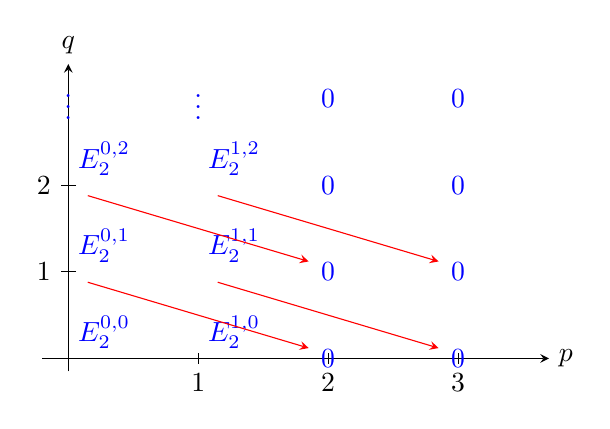
\begin{tikzpicture}[x=1.65cm,y=1.1cm,>=stealth]
\draw[->](-.2,0)--(3.7,0) node[right]{$p$};
\draw[->](0,-.15)--(0,3.4) node[above]{$q$};
\foreach \x in {1,2,3}{\draw(\x,.06)--(\x,-.06) node[below]{$\x$};}
\foreach \y in {1,2}{\draw(.06,\y)--(-.06,\y) node[left]{$\y$};}
\foreach \x in {0,1}{\foreach \y in {0,1,2}{\node[anchor=south west,text=blue] at (\x,\y){$E_2^{\x,\y}$};}}
\foreach \x in {2,3}{\foreach \y in {0,1,2,3}{\node[text=blue] at (\x,\y){$0$};}}
\foreach \x in {0,1}{\node[text=blue] at (\x,3){$\vdots$};}
\foreach \x in {0,1}{\foreach \y in {1,2}{\draw[->,red](\x+.15,\y-.12)--(\x+1.85,\y-.88);}}
\end{tikzpicture}
\]
置 $T_C=\mathcal H om_{\mathcal O_C}(\Omega_C,\allowbreak \mathcal O_C)$, 相应的低次项正合列是
\begin{equation}\label{src:6.3.27}
\begin{aligned}
0\to\underbrace{\mathrm H^1(C,T_C)}_{E_2^{1,0}}&\to\operatorname{Ext}^1_{\mathcal O_C}(\Omega_C,\mathcal O_C)\\
&\to\underbrace{\mathrm H^0(C,\mathcal E xt^1_{\mathcal O_C}(\Omega_C,\mathcal O_C))}_{E_2^{0,1}}\to\underbrace{\mathrm H^2(C,T_C)=0}_{E_2^{2,0}}.
\end{aligned}
\end{equation}
由于 $\Omega_C$ 在结点以外局部自由, $\mathcal E xt^1_{\mathcal O_C}(\Omega_C,\allowbreak \mathcal O_C)$ 和 $\mathcal E xt^2_{\mathcal O_C}(\Omega_C,\allowbreak \mathcal O_C)$ 是仅支撑在 $C$ 的结点 $\Sigma=\{q_1,\allowbreak \ldots,\allowbreak q_s\}$ 上的零维层. 因而 $E_2^{1,\allowbreak 1}=\mathrm H^1(C,\allowbreak \mathcal E xt^1_{\mathcal O_C}(\Omega_C,\allowbreak \mathcal O_C))=0$, 且
\[
\begin{aligned}
E_2^{0,1}&=\mathrm H^0(C,\mathcal E xt^1_{\mathcal O_C}(\Omega_C,\mathcal O_C))\\
&=\bigoplus_j\operatorname{Ext}^1_{\widehat{\mathcal O}_{C,q_j}}(\Omega_{\widehat{\mathcal O}_{C,q_j}},\widehat{\mathcal O}_{C,q_j}),\\
E_2^{0,2}&=\mathrm H^0(C,\mathcal E xt^2_{\mathcal O_C}(\Omega_C,\mathcal O_C))\\
&=\bigoplus_j\operatorname{Ext}^2_{\widehat{\mathcal O}_{C,q_j}}(\Omega_{\widehat{\mathcal O}_{C,q_j}},\widehat{\mathcal O}_{C,q_j}).
\end{aligned}
\]
为计算 $\operatorname{Ext}^i_{\widehat{\mathcal O}_{C,\allowbreak q_j}}(\Omega^1_{\widehat{\mathcal O}_{C,\allowbreak q_j}},\allowbreak \widehat{\mathcal O}_{C,\allowbreak q_j})$, 可假设 $k$ 代数闭. 考虑 $\widehat{\mathcal O}_{C,\allowbreak q_j}=k[[x,\allowbreak y]]/(xy)$ 的局部自由消解
\[
0\to\widehat{\mathcal O}_{C,q_j}\xrightarrow{\binom{y}{x}}\widehat{\mathcal O}_{C,q_j}^{\oplus2}\xrightarrow{(dx,dy)}\Omega_{\widehat{\mathcal O}_{C,q_j}}\to0.
\]
这说明 $\operatorname{Ext}^1_{\widehat{\mathcal O}_{C,\allowbreak q_j}}(\Omega_{\widehat{\mathcal O}_{C,\allowbreak q_j}},\allowbreak \widehat{\mathcal O}_{C,\allowbreak q_j})=\operatorname{coker}(\widehat{\mathcal O}_{C,\allowbreak q_j}^{\oplus2}\xrightarrow{(x,\allowbreak y)}\widehat{\mathcal O}_{C,\allowbreak q_j})=k$, 且 $\operatorname{Ext}^2_{\widehat{\mathcal O}_{C,\allowbreak q_j}}(\Omega_{\widehat{\mathcal O}_{C,\allowbreak q_j}},\allowbreak \widehat{\mathcal O}_{C,\allowbreak q_j})=0$. 前者说明 $\dim_k E_2^{0,\allowbreak 1}=|\Sigma|$ 是结点数; 后者说明 $\operatorname{Ext}^2_{\mathcal O_C}(\Omega_C,\allowbreak \mathcal O_C)=0$, 因为 $E_2^{0,\allowbreak 2}=E_2^{1,\allowbreak 1}=E_2^{2,\allowbreak 0}=0$.

利用短正合列~\bookeqref{6.3.27}, 以及恒等式 $\mathrm H^0(C,\allowbreak T_C)=\operatorname{Ext}^0_{\mathcal O_C}(\Omega_C,\allowbreak \mathcal O_C)$ 和 $\mathrm H^i(C,\allowbreak T_C)=\mathrm H^i(\widetilde C,\allowbreak T_{\widetilde C}(-\widetilde\Sigma))$ (见习题~\bookref{6.2.22}), 有
\[
\begin{aligned}
&\dim_k\operatorname{Ext}^1_{\mathcal O_C}(\Omega_C,\mathcal O_C)-\dim_k\operatorname{Ext}^0_{\mathcal O_C}(\Omega_C,\mathcal O_C)\\
&\qquad=|\Sigma|-\chi(C,T_C)=|\Sigma|-\chi(\widetilde C,T_{\widetilde C}(-\widetilde\Sigma)).
\end{aligned}
\]
将正规化 $\widetilde C=\coprod_{i=1}^{\nu}\widetilde C_i$ 写为连通分支的并, 设 $\widetilde\Sigma$ 为结点轨迹 $\Sigma\subseteq C$ 的原像, $\widetilde\Sigma_i=\widetilde C_i\cap\widetilde\Sigma$. 应用 Riemann--Roch 得
\[
\begin{aligned}
|\Sigma|-\chi(\widetilde C,T_{\widetilde C}(-\widetilde\Sigma))
&=|\Sigma|-\sum_{i=1}^{\nu}\chi(\widetilde C_i,T_{\widetilde C_i}(-\widetilde\Sigma_i))\\
&=|\Sigma|+\sum_{i=1}^{\nu}(3g(\widetilde C_i)-3+|\widetilde\Sigma_i|)\\
&=3\left(\sum_{i=1}^{\nu}g(\widetilde C_i)-\nu+|\Sigma|\right)=3g-3,
\end{aligned}
\]
其中使用了亏格公式 (\bookref{6.2.12}) $g=\sum_{i=1}^{\nu}g(\widetilde C_i)-\nu+|\Sigma|+1$. 这完成无标记点预稳定曲线情形下 (1)--(3) 的证明.

有标记点时, 令 $D=\{p_1,\allowbreak \ldots,\allowbreak p_n\}\subseteq C$. 对短正合列 $0\to\mathcal O_C(-\sum_i p_i)\to\mathcal O_C\to\mathcal O_D\to0$ 应用 $\operatorname{Hom}_{\mathcal O_C}(\Omega_C,\allowbreak -)$, 得到长正合列
\[
\begin{aligned}
0&\to\operatorname{Ext}^0_{\mathcal O_C}(\Omega_C(\sum_i p_i),\mathcal O_C)\to\operatorname{Ext}^0_{\mathcal O_C}(\Omega_C,\mathcal O_C)\\
&\to\operatorname{Ext}^0_{\mathcal O_C}(\Omega_C,\mathcal O_D)\to\operatorname{Ext}^1_{\mathcal O_C}(\Omega_C(\sum_i p_i),\mathcal O_C)\\
&\to\operatorname{Ext}^1_{\mathcal O_C}(\Omega_C,\mathcal O_C)\to0\to\operatorname{Ext}^2_{\mathcal O_C}(\Omega_C(\sum_i p_i),\mathcal O_C)\to0,
\end{aligned}
\]
这里利用了 $i=1,\allowbreak 2$ 时 $\operatorname{Ext}^i_{\mathcal O_C}(\Omega_C,\allowbreak \mathcal O_D)=0$, 因为 $D$ 零维. 由此 $\operatorname{Ext}^2_{\mathcal O_C}(\Omega_C(\sum_i p_i),\allowbreak \mathcal O_C)=0$. 此外, 由于 $\dim_k\operatorname{Hom}_{\mathcal O_C}(\Omega_C,\allowbreak \mathcal O_D)=n$, 已计算无标记点情形的 Ext 群维数之差, 上述长正合列给出
\[
\begin{aligned}
&\dim_k\operatorname{Ext}^1_{\mathcal O_C}(\Omega_C(\sum_i p_i),\mathcal O_C)-\dim_k\operatorname{Ext}^0_{\mathcal O_C}(\Omega_C(\sum_i p_i),\mathcal O_C)\\
&\quad=\dim_k\operatorname{Ext}^1_{\mathcal O_C}(\Omega_C,\mathcal O_C)-\dim_k\operatorname{Ext}^0_{\mathcal O_C}(\Omega_C,\mathcal O_C)+n=3g-3+n.
\end{aligned}
\]
最后, 设 $(C,\allowbreak p_i)$ 稳定, 带标记正规化为 $(\widetilde C,\allowbreak \widetilde p_i,\allowbreak \widetilde\Sigma)$. 习题~\bookref{6.2.22} 说明
\[
\operatorname{Hom}_{\mathcal O_C}(\Omega_C(\sum_i p_i),\mathcal O_C)\cong\operatorname{Hom}_{\mathcal O_{\widetilde C}}(\Omega_{\widetilde C}(\sum_i\widetilde p_i+\widetilde\Sigma),\mathcal O_{\widetilde C}).
\]
由于带标记正规化光滑, 且每个带标记连通分支稳定 (习题~\bookref{6.3.7}), $T_{\widetilde C}(-\sum_i\widetilde p_i-\widetilde\Sigma)$ 在 $\widetilde C$ 的每个连通分支上的次数严格为负. 因而 $\operatorname{Hom}_{\mathcal O_C}(\Omega_C(\sum_i p_i),\allowbreak \mathcal O_C)=0$. 另见~\cite[命题 1.5]{DM69} 和~\cite[\S 11.3]{ACG11}.
\end{proof}
上述证明还揭示了整体与局部形变的重要关系. 用 $\operatorname{Def}(C,\allowbreak p_i)$ (分别地, $\operatorname{Def}^{\mathrm{lt}}(C,\allowbreak p_i)$) 表示 $(C,\allowbreak p_i)$ 的一阶形变 (分别地, 局部平凡一阶形变) 的向量空间.
\begin{proposition}[从局部到整体的形变序列]\label{src:6.3.28}
设 $(C,\allowbreak p_i)$ 是代数闭域 $k$ 上的 $n$-点预稳定曲线, $\Sigma\subseteq C$ 是结点集. 设 $\pi:\widetilde C\to\allowbreak C$ 是正规化, $\widetilde p_i$ 是 $p_i$ 的唯一原像, $\widetilde\Sigma=\pi^{-1}(\Sigma)$. 有正合列
\begin{equation}\label{src:6.3.29}
0\to\operatorname{Def}^{\mathrm{lt}}(C,p_i)\to\operatorname{Def}(C,p_i)\to\bigoplus_{q\in\Sigma}\operatorname{Def}(\widehat{\mathcal O}_{C,q})\to0
\end{equation}
及等同
\[
\begin{aligned}
\operatorname{Def}^{\mathrm{lt}}(C,p_i)&\cong\mathrm H^1(C,T_C)\\
&\cong\mathrm H^1(\widetilde C,T_{\widetilde C}(-\sum_i\widetilde p_i-\widetilde\Sigma))\cong\operatorname{Def}(\widetilde C,p_i,\widetilde\Sigma),\\
\operatorname{Def}(C,p_i)&\cong\operatorname{Ext}^1_{\mathcal O_C}(\Omega_C(\sum_i p_i),\mathcal O_C),\\
\operatorname{Def}(\widehat{\mathcal O}_{C,q})&\cong\operatorname{Ext}^1_{\widehat{\mathcal O}_{C,q}}(\Omega^1_{\widehat{\mathcal O}_{C,q}},\widehat{\mathcal O}_{C,q})\cong k,\qquad q\in\Sigma.\quad\square
\end{aligned}
\]
\end{proposition}
\begin{exercise}[再论稳定曲线的形变]\label{src:6.3.30}
\begin{enumerate}[(a)]
\item 直接证明无标记点稳定曲线的形变无障碍.

\textit{提示:} 设 $q_i\in C$ 为结点, 取仿射开集覆盖 $C=U_1\cup U_2$, 使得每个 $q_i\in U_2\setminus U_1$. 利用 $U_1$ 和 $U_{12}=U_1\cap U_2$ 无障碍 (因为光滑), 且 $U_2$ 也无障碍 (因为是仿射局部完全交, 参见命题~\bookref{A.3.7}), 证明 $U_1,\allowbreak U_{12},\allowbreak U_2$ 的形变可粘合成 $C$ 的形变. 另见~\cite[Tag 0DZQ]{SP}.
\item 将论证推广到有标记点的情形.
\item 能否改用余切复形的性质证明?
\end{enumerate}
\end{exercise}
\begin{remark}[形变理论的推论]\label{src:6.3.31}
很快将知道 $\overline{\mathcal M}_{g,\allowbreak n}$ 是代数叠, 然后可用形变理论说明它是维数为 $3g-3+n$ 的光滑 Deligne--Mumford 叠 (见定理~\bookref{6.4.16}). 核心思想如下:
\begin{itemize}
\item $\operatorname{Ext}^0$: 已知稳定曲线 $(C,\allowbreak p_i)$ 只有有限多个自同构 (命题~\bookref{6.3.5}). $\operatorname{Ext}^0$ 消失说明 $n$-点稳定曲线 $(C,\allowbreak p_i)$ 没有无穷小自同构, 即自同构群概形 $\underline{\operatorname{Aut}}(C,\allowbreak p_i)$ 约化, 有限且平展. 由此可用 Deligne--Mumford 叠的刻画 (\bookref{4.6.4}) 得到 $\overline{\mathcal M}_{g,\allowbreak n}$ 是 Deligne--Mumford 的.
\item $\operatorname{Ext}^1$: 它参数化域 $k$ 上的稳定曲线 $(C,\allowbreak p_i)$ 的形变同构类, 因而等同于 $\overline{\mathcal M}_{g,\allowbreak n}\times_{\mathbb Z}k$ 在对应于 $(C,\allowbreak p_i)$ 的 $k$-点处的 Zariski 切空间. $\operatorname{Ext}^1$ 的计算说明 $\overline{\mathcal M}_{g,\allowbreak n}$ 在 $\Spec\mathbb Z$ 上的相对维数为 $3g-3+n$.
\item $\operatorname{Ext}^2$: 它的消失说明 $(C,\allowbreak p_i)$ 的形变没有障碍, 因而无穷小提升判据 (\bookref{4.7.1}) 说明 $\overline{\mathcal M}_{g,\allowbreak n}$ 在 $\Spec\mathbb Z$ 上光滑.
\end{itemize}
\end{remark}
